\documentclass[10pt]{article}
\usepackage[margin=0.7in]{geometry}
\usepackage[T1]{fontenc}
\usepackage{lmodern,amsmath,graphicx,booktabs,hyperref}
\hypersetup{colorlinks=true,urlcolor=blue}
\setlength{\parindent}{0pt}\setlength{\parskip}{5pt}
\setlength{\emergencystretch}{3em}
\begin{document}
{\Large\bfseries The active leaf guard supplies the size comparison}

23 November 2026. Classical/local only; no S3.
Formal record PCC85abe4 is unsigned. \texttt{[pcc:unverified]}

The actual Setup stores leaf\_size$=\lfloor s/q\rfloor$, with
$q=\max(k,1)>0$. The parameter routine first rejects
$M\le\lfloor s/q\rfloor$. A call passing that size guard therefore satisfies
\[
 \lfloor s/q\rfloor<M \quad\Longrightarrow\quad s<Mq
 \quad\Longrightarrow\quad s\le Mq.
\]
The first implication is exactly Std's existing
\texttt{Nat.div\_lt\_iff\_lt\_mul}; the second weakens strict order.
This is a source-bound application, not a new division theorem.

\textbf{Precision application.} The existing shared conditional34 theorem
requires hroot:$s\le Mq$. The consumer now supplies that premise from the
source size guard. Every other premise remains explicit:
\[
 u\le M,\quad i<u,\quad p\le cs2^A,\quad cqu\le2^{u+1},\quad
 8u(A+2u+1)\le2^{A+u+1}.
\]
The conclusion remains
$u\,\mathrm{childPrecision}(p,M,u,A+2u,i)\le34M2^{A+2u-i}$.
Here $p$ denotes ring precision. Neither inherited precision nor the
dimension conditions are inferred from activity. No lower child-size bound
is inferred from the separate shrinkage upper bound.

\begin{center}
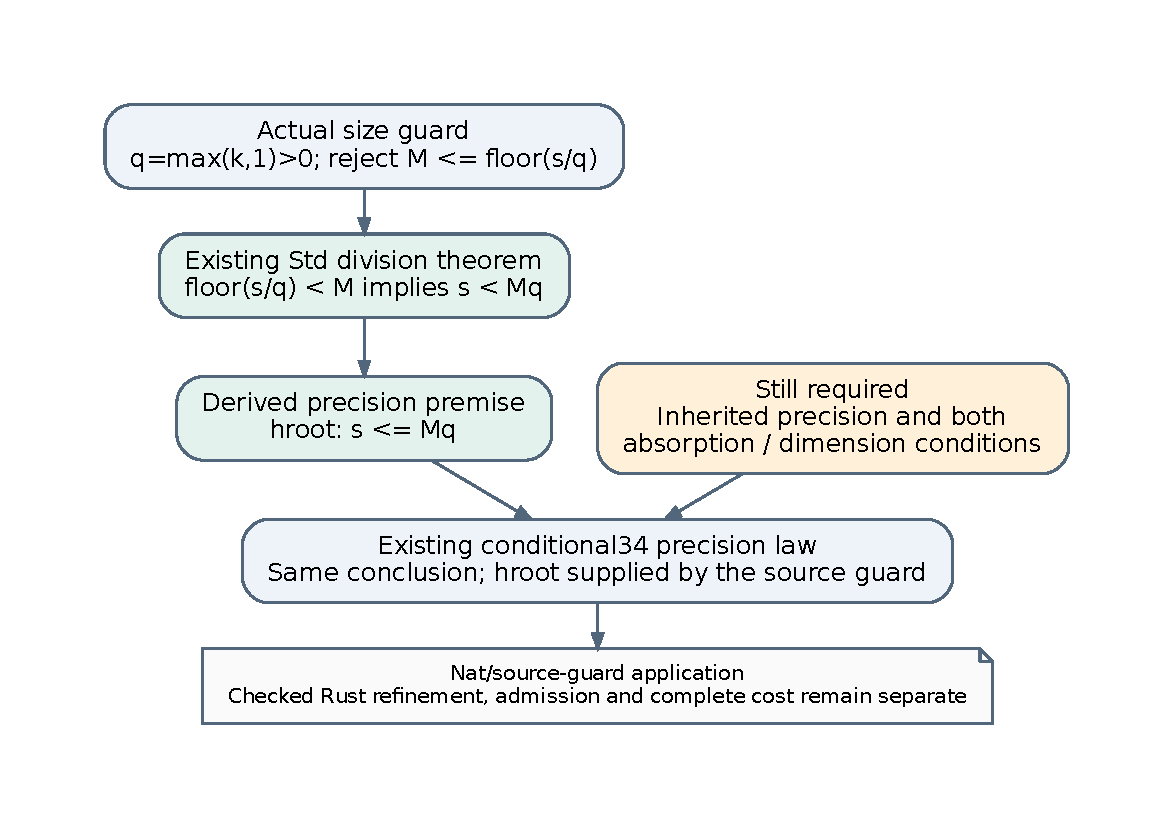
\includegraphics[width=0.95\linewidth,height=3.7in,keepaspectratio]{guard.pdf}
\end{center}

\textbf{Exact source scope.} k may be any natural in the proof; the source
chooses floor\_sqrt(lambda), then takes max with1. Passing the size guard
does not imply that the degree, scale, array and checked-width conditions
also pass. This is not a machine-checked Rust refinement or production
admission theorem. Current64-bit usize root\_u remains0. The actual source's
floor division is kept distinct from the primary paper's rounded-up threshold.

\newpage
{\large\bfseries Qualification, controls and remaining obligations}

One source-frozen qualification privately recompiles the unchanged shared
owner, then the consumer. The unchanged proof gates audit seven consumer
and three existing owner declarations, with zero trusted native proofs.
Official \texttt{leanchecker --fresh LeafGuard} exits0. Eight explicit axiom
queries use only propext/Quot.sound; three literal controls use no axioms.
These are unsigned producer observations, not signed standing or independent
execution. Imports are Std-only, on official Lean4.35.0.

\begin{tabular}{p{0.30\linewidth}p{0.64\linewidth}}
\toprule
Scope control & Kernel-checked fact\\\midrule
Drop activity &s=3,M=1,q=2: activity false and $s\le Mq$ false\\
Allow zero divisor &Nat gives $1/0<1$, but $1<1\cdot0$ is false\\
Inactive divisible boundary &$4/2=2$, $4\le2\cdot2$, but not $4<2\cdot2$\\
Nonempty scalar application &p=1,M=16,u=12,A=i=0,s=24,k=2,c=1; all other scalar premises hold\\
\bottomrule
\end{tabular}

The boundary example prevents treating the weaker conclusion as equivalent
to activity. The nonempty application is deliberately not Setup-admitted
recursion. Small controls clarify scope; the universal result applies the
existing division and precision theorems. No new native or solver run occurs.

\textbf{Evidence and method.} The six-field instance map preceded the first
Lean edit. No missing generic component was found, so no owner theorem was
replaced or rederived. Kernel source is pinned to official Lean4.35.0;
the exact shared owner is crypto-lean50b95696, and native Setup source is
crypto76969347. Source/command hashes and all outputs are retained.
Qualification exits0/physicalstop0 and peaks at14373085184bytes under the
unchanged15032385536-byte sampled stop. One compiler worker and600s phase
ceilings stay fixed. No raised elaboration limit, custom axiom, hole or
native\_decide is used.

\textbf{Prior sources.} Read the exact Std division theorem in
Init/Data/Nat/Div/Basic.lean:314, actual Setup methods, the existing shared
precision theorem, pinned primary AppendixD.11 and the October30 cost review.
The latter already uses active leaf thresholds in inherited-precision
accounting. KB MCP is absent; two mechanism/negative searches and theorem
lookup each return127. Bounded GitHub fallback supplies source pointers,
not novelty or absence clearance.

\textbf{What remains.} Source-history inherited precision, both dimension
conditions, checked Rust refinement and complete bit cost remain separate
obligations. The prior root35, conditional34 and history laws are unchanged.
The port/vertex study, original native controls and CPU baseline remain intact.
Shared-repository default-Mathlib/whole-library integration and signed standing
are not established by this Std-only application. Canonical timing charts and
rankings are unchanged for this mathematical component.

\textbf{Reproduction.} Compile the exact shared source into a private
CryptoLeanCore import directory, compile LeafGuard, run the unchanged gate on
both files, inspect all eight axiom queries, then use the official fresh
checker. The local checkpoint retains sources, objects, commands, receipts
and precise next action. No S3 upload is used.

\small Full prospective map, declaration bindings, checked source identities,
scope controls and qualification outputs accompany this report.\par
\url{https://github.com/isogeny-labs/crypto/pull/5046}\par
\url{https://github.com/aburan28/crypto-lean/blob/50b95696db2e7a34b7c5f1ba47eb5408f49ca12d/CryptoLeanCore/TaperedPrecision.lean}
\end{document}
